\documentclass{sig-alternate}

\usepackage{listings}
\usepackage{graphicx}   
\usepackage{subcaption}   % for subfigure
\usepackage[color]{coqdoc}
\usepackage{lstlangcoq}
\usepackage{booktabs}
\usepackage{balance} %For balancing the last page
\usepackage{caption}
\usepackage[ruled,vlined,linesnumbered]{algorithm2e}
\usepackage{algorithmic}
\usepackage{fancyvrb,floatrow}
\usepackage{inputenc}
\usepackage[T1]{fontenc}
\usepackage{amsmath,amssymb}
\usepackage{pdfpages}
\usepackage{color,soul}
\usepackage{cite} %For citations
\usepackage{todonotes} %For comments
\usepackage{hyperref} %For correctly depicting urls

\let\proof\relax
\let\endproof\relax
\usepackage{amsthm} %For theorems
\usepackage{multirow} %For spanning a cell into multiple rows 
\usepackage{rotating} %For rotating text inside the table
\usepackage{bigstrut} %For leaving an extra bit of space between text and the table border
\usepackage{courier} %For courier font
\usepackage{tikz}
\usetikzlibrary{matrix,arrows}
\usetikzlibrary{shapes.geometric}
\usepackage{verbatim}
\linespread{1.067}

\definecolor{keywords}{RGB}{127,0,85}
\definecolor{comments}{RGB}{19,121,0}
\definecolor{strings}{RGB}{0,0,255}
\definecolor{light-gray}{gray}{0.80}

\hypersetup{
    colorlinks,
    linkcolor=black,
    citecolor=black,
    urlcolor=black
 }

\begin{document}
% Copyright
\setcopyright{acmcopyright}
%\setcopyright{acmlicensed}
%\setcopyright{rightsretained}
%\setcopyright{usgov}
%\setcopyright{usgovmixed}
%\setcopyright{cagov}
%\setcopyright{cagovmixed}
% \acmPrice{\$15.00}

%\def \@covert{{\emph {\large C}}{\emph{\normalsize OVERT}}}

\title{\textbf{{\huge A}{\LARGE STRONAUT:}} %Astronaut: %A Framework for Dynamic Tradespace Analysis
A General Algebraic Theory and Derived Software Framework for Automated Tradeoff Analysis}
% \numberofauthors{3}
% \author{
% % 1st. author
% \alignauthor
% Chong Tang\\
% \affaddr{University of Virginia}\\
% \affaddr{Charlottesville, VA 22904}\\
% \email{ctang@virginia.edu}
% % 2nd. author
% \alignauthor
% Kevin Sullivan\\
% \affaddr{University of Virginia}\\
% \affaddr{Charlottesville, VA 22904}\\
% \email{sullivan@virginia.edu}
% %3rd author
% \alignauthor
% Hamid Bagheri\\
% \affaddr{University of California, Irvine}\\
% \affaddr{Irvine, CA 92697}\\
% \email{hamidb@uci.edu}
% }


\newcommand{\superscript}[1]{\ensuremath{^{\textrm{#1}}}}
\def\sharedaffiliation{\end{tabular}\newline\begin{tabular}{c}}

\def\wu{\superscript{*}}
\def\wg{\superscript{\S}}%\dag}}

\numberofauthors{1}
\author{
  \alignauthor \ Chong Tang\wg~~~~~~~~~Hamid Bagheri\wu~~~~~~~~~~Sarun Paisarnsrisomsuk\wg~~~~~~~~~~Kevin Sullivan\wg\\
% ctang@virginia.edu~~bagheri@unl.edu~~~~~~sullivan@virginia.edu~~~~~~sp4et@virginia.edu
  %\email{hb2j@virginia.edu}
  %
%  \alignauthor \ Chong Tang\wg\\
%  \email{ctang@virginia.edu}
  %
%  \alignauthor Kevin Sullivan\wg\\
%  \email{sullivan@virginia.edu}
  %
%  \alignauthor Kevin Sullivan\wg\\
%  \email{sullivan@virginia.edu}
  %
  \sharedaffiliation
  \begin{tabular}{ccc}
    \affaddr{{\wg}Computer Science Dept.{\ }} & & \affaddr{{\wu}Computer Science and Engineering Dept.{\ }} \\
    \affaddr{University of Virginia}            & & \affaddr{University of Nebraska} \\
    \affaddr{Charlottesville, VA 22903.}            & & \affaddr{Lincoln, NE 68510. } \\
    \affaddr{\{ctang,sp4et,sullivan\}@virginia.edu{\ }} & & \affaddr{bagheri@unl.edu{\ }} \\  
%    \affaddr{United States}                  & & \affaddr{United States} \\
  \end{tabular}
} 
    

\maketitle
\begin{abstract}
\sloppy
Abstract, thus partial, system specifications give rise to tradespaces: sets of designs that satisfy specified constraints, yet vary in other, often non-functional, properties. Exploring such spaces to find high-value solutions is hard and time-consuming. The current state-of-the-art in software engineering still provides inadequate support for efficient tradespace analysis. 
In this paper, we present to our knowledge the first scientific foundations and a novel, general-purpose software technology, \textsc{Astronaut}, for practical analysis of system properties, tradeoffs, and value. We formally express our model of tradespace analysis in the constructive logic of Coq, and automatically derive the Scala implementation of \textsc{Astronaut} directly from this specification. \textsc{Astronaut} not only enumerates design models for a given specification, but converts them to implementations, runs them, profiles their performance in multiple dimensions, and presents the resulting tradespace profile in useful forms. It can be instantiated for use in various domains.
Our experience with using \textsc{Astronaut} in the context of object-relational database mappings corroborates its ability to reveal designs that greatly outperform %those that current tools and methods tend to produce.
those produced by %widely-used, industrial tools.
state-of-the-art methods for database schema synthesis.

\begin{comment}
 %and assessed its function and performance as we used it to carry out the experiments reported herein.

The main contribution of this paper is the first experimental evidence that, in one important domain, the {\em relational-logic-based  tradespace analysis} (RLTA) tends to reveal designs that are are significantly better than those that standard methods produce. These experiments required a new apparatus: the second contribution of this work. Called {\em Astronaut,} it is an object-oriented framework for {\em dynamic} RLTA. It not only enumerates design models for a given specification, but converts them to implementations, runs them, profiles their performance in multiple dimensions, and presents the resulting {\em tradespace profile} in useful form. It can be instantiated for use in various domains. The third contribution of this work is a formal specification of Astronaut. It expresses our model of tradespace analysis in the constructive logic of Coq. We extracted the Scala implementation of Astronaut directly from this specification and assessed its function and performance as we used it to carry out the experiments reported herein. 
%It is parameterized by a domain-specific specification language, semantics, and set of dynamic property measurement functions, provided as subclasses of framework classes. Astronaut automates end-to-end mapping of specifications through exhaustively enumerated design spaces to complete dynamic tradespace profiles. We adapted results of prior work of Bagheri et al. to instantiate Astronaut for the object-relation mapping domain and used it to run the experiments reported here. Astronaut uses Alloy as a model finder. While model enumeration is a scale-limited {\em \#P-complete} problem, profiling implementations is trivially parallelizable. Astronaut uses a Spark-based cluster to profile implementations in parallel, reducing profiling times for our experiments from weeks on a personal computer to just a few minutes. Concretely, our work suggests that standard ORM tools tend to produce vastly performance-suboptimal databases. 


%We hypothesize that efficient systematic tradespace modeling and analysis could reveal designs that greatly outperform those that current tools and methods tend to produce. 
Our experience with using \textsc{Astronaut} in the context of object-relational database mappings corroborates its ability to reveal designs that greatly outperform %those that current tools and methods tend to produce.
those produced by %widely-used, industrial tools.
state-of-the-art methods for database schema synthesis.
\end{comment}

\end{abstract}

%\begin{abstract}
%Abstract, thus partial, system specifications give rise to {\em design spaces}: sets of designs that satisfy specified constraints but that vary in other properties. The hypothesis driving work on design space tradeoff analysis (DSTA) is that {\em in practice, systematic analysis of the properties of designs across such spaces tends to reveal designs with better tradeoffs than those that designers would otherwise achieve.} The primary contribution of this paper is the first experimental test of the validity of this hypothesis for the {\em relational-logic-based DSTA method of Bagheri et al.} (RL-DSTA). We present evidence from several experiments suggesting that, at least in the domain of object-oriented-to-relational-database mapping (ORM) tools, RL-DSTA does tend to reveal designs that are are strictly and significantly better than those that produced by commercial ORM tools, and that finding such designs using RL-DSTA is practical for data model specifications at modest scales that have proven useful in practice. Carrying out these experiments required a novel automated apparatus: not only to enumerate design models but to convert them to executable implementations, to profile their performance under controlled loads given specific dynamic (runtime) property measurement procedures, and to manage the resulting data. The second result of this work is a system for this purpose: {\em Astronaut}. It is a formally specified, general-purpose, object-oriented framework for {\em dynamic} RL-DSTA. It  fully automates the end conversion of system specifications into dynamically profiled tradespaces. To test its usability and utility, we specialized it to the ORM domain and used it carry out our experiments. These uses involved profiling of design spaces with tens or hundreds of thousands of designs. As a framework Astronaut is parameterized by specification language, semantics, and dynamic property measurement functions, which are provided as subclasses of core framework classes. While exhaustive, bounded relational logic model enumeration is a {\em \#P-complete} problem, thus inherently scale-limited in general, profiling model implementations is trivially parallelizable. We made Astronaut practical by incorporating a Spark-based back-end for scalable, parallel profiling of the large numbers of designs typically generated by RL-DSTA even from modest-sized specifications, reducing profiling time from weeks to hours or minutes.
%\end{abstract}

\def \@approach{\textsc{Astronaut}}
%{\normalsize A}{\small OVERT$^{+}$}}

\keywords{design space; synthesis; tradespace; dynamic analysis; relational logic; experimental software engineering}

% \section{Cut Stuff}

% Bagheri et al. recently presented an automated DSTA method based on the following:

% Such PPDs map {\em design models} to predicted property values, such as runtime performance. As a test of potential utility, Bagheri et al. conducted an experiment in the domain of object-relational mapping. Specifications expressed object-oriented data models; the semantics specified possible object-relational mappings; and design solutions represented SQL schemas. Their main result was a statistical test of the accuracy of a set of previously published runtime database performance PPDs based on a comparison of predicted time and space performance properties against actual performance determined by profiling concrete implementations under load for a sample of the designs in the design space. What Bagheri et al. did not do is to directly test their approach against the 

%In previous work, we presented an approach to synthesize software designs, and manually conducted limited dynamic analysis on some sampled designs. The results showed that static estimators of runtime database performance are not accurate. Our previous work left some important questions unanswered: (1) what are the actual tradeoff curve and the Pareto-optimal designs, (2) whether our synthesis and tradeoff profiling method has potential to reveal better software designs than commonly used tools and methods. To answer these questions, we need to conduct fully exhaustive analysis for all designs in a tradeoff space. We were unable to answer them due to lack of tool support. In this work, we designed and implemented a generalized and automated tradeoff space synthesis and tradeoff profiling infrastructure. We first produced a generic formal specification of the framework in Coq. Then we extracted Coq to Scala to produce an executable implementation in the form of an object-oriented framework that is easy to specialize by subclass extension. We partially demonstrated the generalization by instantiating this framework into a tool in object-relational mapping domain. We used this tool to synthesize database schemas from specifications, conduct dynamical analysis of synthesized schemas, and select design based on the analysis result. Our findings show that our method can find practical far better solutions than those produced by ordinary means.

\section{Introduction}
Specifications are generally incomplete with respect to design details and the totality of desirable system properties, many of which often depend on the choice of design. For example, while an object-oriented data model, as a specification, constrains the behavior of a persistent data store, it does not uniquely determine the database schema (design); nor does it express preferences for performance properties or tradeoffs involving read and write times and file sizes, which, in general, can vary greatly with the choice of schema. 

%Incomplete specifications thus 
Unspecified or underspecified properties create degrees of freedom that
give rise to {\em tradespaces:} sets of designs that satisfy a given specification but that vary in other relevant properties (often non-functional properties such as time and space performance, reliability, and evolvability). An engineer then has two choices. %The {\em default approach} is %to accept some readily producible design as {\em good enough.} 
The \textit{single-point strategy} is
to use design heuristics, tacit knowledge, and other such methods in developing point solutions that, it is hoped, will be good enough for stakeholders in all key dimensions.
 
%The default approach is often supported by design {\em methodologies,} tools, or even just training and experience. Such methods work by making default design decisions that are generally expected to produce {\em good enough} results. The benefit is that this approach relieves the engineer of having to engage in a more demanding TA process. The disadvantage is that it can produce designs that are significantly, even dramatically, worse than could be obtained using TA. 

\sloppy The single-point strategy is often supported by design methodologies, tools, or even just training and experience.
%Similarly, 
In fact, when tools automatically produce implementations, they often use single-point strategies. Consider object-relation mapping (ORM) tools, now provided in many programming environments. They map object-oriented data models to relational schemas and code for managing application data. They often use a single mapping strategy, and do not help engineers understand available solutions or the tradeoffs in time and space performance that they entail.

The alternative approach, which we call {\em tradespace analysis strategy}, is to consider design spaces, estimate or measure their properties,  then choose one that realizes a desirable set of properties. 
The fundamental {\em hypothesis} driving the development and use of systematic and automated tradespace analysis is that {\em it produces results of greater value even net of its additional costs}. %This hypothesis has two parts. The first component hypothesis is that, {\em in domains where it is applicable, 
Indeed, tradespace analysis tends to reveal designs, that otherwise engineers might miss, with properties and tradeoffs that are significantly better than those that engineers would otherwise obtain (e.g., using single-point methods). %The second component hypothesis is that {\em these value of the improvements outweigh the added costs of TA.}


In this paper, we present scientific foundations and a general-purpose software technology, dubbed \@approach, for practical analysis of system properties, tradeoffs, and value. We leverage recent advancements in several areas, such as constructive logic, formal synthesis and scalable big data analytics, to develop such a novel technology base.
More specifically, this paper contributes a formal, general algebraic theory of design space tradeoff analysis tools, and a map-reduce-based framework, derived mechanically from the theory, for implementing such tools. The theory is organized as a hierarchy of Coq typeclasses. From this theory, we automatically derive a polymorphic framework (in Scala) that developers specialize and extend to produce domain-specific trade-off analysis tools.

%\newpage
As a test and demonstration, we instantiated this framework to create an automation tool %that supports tradeoff analysis in the context of object
for carrying out tradespace analysis in the context of the object-relation mapping domain.
Our experimental results strongly suggest that % industrial object-relation-mapping synthesis tools, such as Rails and Django, tend to produce results that are surprisingly worse than designs discovered by our method. 
\@approach tradespace analysis enables production of database designs that significantly outperform those produced by %widely-used, industrial ORM tools
industrial ORM synthesis tools, such as Rails and Django, yet are entirely overlooked by such widely-used, industrial tools. %state-of-the-art methods for database schema synthesis.

\begin{comment}
\@approach tradespace analysis enables production of database designs that are entirely overlooked by %widely-used, industrial ORM tools
industrial object-relation-mapping synthesis tools, such as Rails and Django, yet greatly outperform those produced by such widely-used, industrial tools. %state-of-the-art methods for database schema synthesis.
\end{comment}

%As a test and demonstration, we instantiated this framework using code re-engineered from an earier, ad hoc, only partially automated system for tradeoff analysis of object-relation mappings. Our new tool reduced the time taken by one analysis from weeks to hours.

%This paper develops a new approach to implement systems gave incomplete specifications through a case study operating at two levels. At a high level, we develop a framework for tools that implement an exhaustive, formal-specification-driven, batch sequential tradespace approach. By batch sequential we mean that we fully evaluate an implementation and only then do we apply property estimation or measurement functions to profile the tradespace. At a lower level, we develop an instance of such a tool for carrying out formal-specification-driven tradespace analysis for the object-relation mapping (ORM) domain mentioned at the start of this paper.

%Our overall hypothesis is that a tradespace exploration and analysis approach tends to produce significantly better results than those produced by widely used ORM tools, many of which implement throw-a-dart assumptions. None that we know of support systematical tradeoff analysis. The main contributions of this work includes a generic model that supports tradespace analysis from incomplete specifications, a tool instantiated from this framework with map-reduce-backed dynamic analysis, and a set of experimental results which strongly support this hypothesis.



To summarize, this paper makes the following contributions:
\begin{itemize}

%\item \textit{A formal theory of tradeoff analysis:}  We present a formal, general, algebraic theory of tradeoff analysis conceptualized in constructive logic.
\item \textit{Theoretical framework:} We develop a theoretical framework conceptualized in constructive logic to make the notion of tradeoff analysis precise.

\item \textit{Tool implementation:} %We show how to exploit the power of our formal abstractions by building a mechanically derived, polymorphic, map-reduce-based, general-purpose framework for, tradeoff analysis tools. 
We show how to exploit the power of our formal abstractions by building a mechanically derived, polymorphic implementation framework for tradeoff analysis tools.  
 

\item \textit{Experimental evaluation:} \sloppy
We present our experiences with thorough evaluation of \@approach in the context of tradeoff analysis of object-relational database mappings, the results of which corroborate that \@approach reveals designs %that are strictly and strikingly better than those produced by widely-used, industrial ORM tools.
that strictly and strikingly outperform those produced by widely-used, industrial ORM tools.

\end{itemize}

\sloppy
%\@approach is available for download along with all benchmarks, documentation and scripts necessary to reproduce our experimental results: http:// /\@approach/

The rest of this paper is organized as follows. 
Section 2 motivates our research through an illustrative example.
Section 3 provides an overview of \@approach.
Section 4, 5 and 6 describe the details of our constructive logic based framework of tradeoff analysis, framework instantiation, and parallelization reasoning, respectively.   
Section 7 presents the evaluation of the research. Finally, the paper concludes with an outline of the related research and our future work.


\begin{comment}

\newpage

The main result of this paper is a body of  evidence, from several laboratory experiments, that supports the validity of the first component hypothesis for one particular TA approach, the {\em relational-logic-based TA} approach of Bagheri et al. ({\em RLTA})~\cite{trademaker}.\footnote{We do not rigorously address the second component hypothesis because its validity depends heavily on the economics of the environment in which a system is developed.} RLTA uses relational logic to define domain-specific specification languages and their non-deterministic semantics, and relational logic model finders to exhaustively enumerate design models for specifications in such languages consistent with their semantics.  

Our evidence suggests that, in the domain of object-to-relational mapping (ORM), where specifications denote OO data models and designs are mappings to relational database schemas, RLTA {\em does} reveal designs that, by our measures, are strictly and {\em strikingly} better than those produced by default industrial ORM tools. This is a new result.

These experiments in turn required a new apparatus. We called it {\em Astronaut}. Astronaut fully automates the end-to-end conversion of system specifications into dynamically profiled tradespaces, i.e., exhaustive {\em dynamic} relational-logic-based tradespace analysis.  Its design and evaluation is the second contribution of this work. The previous work of Bagheri et al. dynamically profiled only a few hundred designs, reportedly at a cost of months of manual effort, to enable statistical testing of the predictive accuracy of certain {\em static} database performance predictors (which operation directly on static design models of SQL schemas).  Astronaut not only enumerates very large numbers of designs (like the prior work), but (unlike that work) converts them into to executable implementations (here, databases), runs them in parallel under load on a Spark cluster, profiles their runtime performance properties using given property measurement procedures, and gathers, analyzes, and presents the resulting data in useful form. 

Astronaut in turn implements an abstract model for TA, presented informally by Bagheri et al. in previous work~\cite{trademaker}. However, they never formalized or mechanically checked their model. The third contribution of this work is a formal specification, written in the logic of Coq and checked for consistency, from which we extracted the Scala implementation of Astronaut. The Coq specification is polymorphic in types that encode the syntax and semantics of a given domain-specific specification language, the solver that will be used to enumerate designs, the set of property estimation or measurement procedures used to profile designs, etc. These parameters are extracted to Scala as abstract classes that are overridden to instantiate Astronaut for a given domain. The earlier technology of Bagheri et al. was hand-crafted and specialized to the ORM domain. Astronaut can be instantiated for many domains. Our work involved re-engineering ORM-specific code of Bagheri et al. into sub-classes that we then plugged into Astronaut to instantiate it as an ORM tool. We  present our Coq specification as a straightforward, abstract, formalized, generalized, and evolvable theory of dynamic TA, from which code can be extracted automatically, and which we have tested for utility by using it to create Astronaut.

A comment on scalability is in order. RLTA, thus Astronaut, involves exhaustive enumeration of models of bounded relational logic models. This is a {\em \#P-complete} problem: harder than {\em NP-complete} and equivalent to counting the number of satisfying solutions to a SAT problem. It is intractable in general, and will not scale to complex, integral systems. Yet model checking tools have clearly demonstrated the potential value in exploring practical uses of solutions to theoretically intractable problems. RLTA is no panacea. It might be useful. Here we remain satisfied to explore its potential utility for problems at the scale of individual modules, such as database schemas for ordinary web applications. While the modular architecture of Astronaut supports variation in logics and solvers thus enumeration strategies, we leave the exploration of such variations on our theme to future work. 

% profiling implementations is trivially parallelizable. We made Astronaut useful by incorporating a Spark-based back-end for parallel profiling of the tens of thousands (or more) of designs found even for modest specifications, reducing dynamic profiling time from weeks on a personal computer to minutes on a cluster.

% The Coq specification provides a foundation for exploring at a declarative level alternatives to the current approach. Examples of alteratives might include systems that trade away complete enumeration of design spaces for tractability on large-scale specifications. 

\end{comment}

%%%%%%%%%%%%%%%%%%%%%%%%%
%%%%%%%%%%%%%%%%%%%%%%%%%
%%%%%%%%%%%%%%%%%%%%%%%%%

%\newpage
\section{Driving Problem}
%\section{Motivation and running example}
\label{problem}

In this section, we discuss how incompleteness in specification gives rise to important separations of concerns and the need for a systematic understanding and application of tradeoff analysis. We then present a running example having to do with tradeoff analysis among the space of possible solution alternatives.

\subsection{Strategic Incompleteness in Specification} Specifications are often incomplete with respect to the full range of properties that stakeholders value in a given system. Such incompleteness is often not a flaw. Rather, it can serve a strategic function in structuring the process of complex system design. When a specification is silent on system properties relevant to stakeholders, it partitions the design process, the representation of acceptable solutions, and the set of design decisions to be made. We address each of these separations of concerns and explain how they create a need for a better theory of and technology for tradeoff analysis.

\textbf{Partitioning of the Design Process.}
Incompleteness partitions the design process into at least two distinct parts. The first is a deductive process, in which candidate solutions are derived from a specification, constrained only by the condition that they satisfy its terms. Such solutions generally differ in stakeholder-relevant properties on which the specification was silent. The second part is thus an optimization process, in which solutions are evaluated for additional properties, tradeoffs are identified, candidates are ranked, and one is selected for use or development.


\textbf{Partitioning of Design Representations.}
This deductive vs. optimization partitioning of the design process is mirrored by an explicit vs. implicit partitioning of the representation of what constitutes an acceptable solution. The explicit part is given by the specification. The implicit part is represented in the property estimation functions that will be used to evaluate solutions, the stakeholder utility functions (emergent or documented) that map property estimates to stakeholder utilities, and the stakeholder tradeoff functions (emergent or documented) that map the multiple stakeholder utilities to a final ranking of, and ultimately to a choice from among, candidate design solutions.  

\textbf{Partitioning of Design Decision Spaces.}
The deductive vs. optimization and explicit vs. implicit dichotomies extend to a split between decisions that are understood and agreed on well enough to be pinned in a specification, and those that are not. This is a split between settled vs. unsettled decisions. A specification speaks explicitly on design decisions that are settled while remaining silent on relevant but as yet unsettled aspects, leaving them to be worked out in downstream, optimization-oriented design activities.

%\textbf{The Evolution of Incompleteness in Design.}
These separations of concerns can also sometimes be seen in the evolution dynamics of complex systems. As initially unsettled concerns are settled, they can migrate from being represented implicitly in measurement and utility functions to being explicit in specifications. System architectures can be seen as settled and explicit specifications, for example, that remain incomplete in other key areas. As optimization-based processes produce knowledge and agreement, these results can migrate into specifications.

\subsection{Running Example}
To further motivate the research and illustrate our approach, here we provide a running example having to do with tradeoff analysis among the space of possible solution alternatives. Consider object-relational database mapping. In ORM domain, a specification is an object model that contains objects and relationships among these objects. Object-oriented data models serve as specifications for application database schemas. %Figure 1 shows a model with three classes and some relations among them. 
While these specifications constrain schemas, they are silent on properties such as time and space performance, and evolvability. At the same time, degrees of freedom in ORM mappings (e.g., in how inheritance is mapped to relations) give rise to spaces of satisfying schemas that vary in these properties. Object-oriented specifications of data models are incomplete regarding these other properties.
While all solution points within the solution space are equally good at satisfying the specification, they will differ in other properties of interest in design.  

Incompleteness is generally resolved today by policies hard-wired into ORM packages. One straightforward solution is created for any given specification, without much consideration of stakeholder preferences. Such tools impose tradeoffs on stakeholders that might or might not be desirable.

The above example points to one of the most prominent and widely-used software/system engineering problems that we take as a running example that requires tradeoff analysis to be addressed effectively.
The upshot is that tradespace analysis is an important part of practical design, in general. The motivation for this paper is the current lack of adequate scientific foundations and technologies for tradespace analysis in software and systems engineering. The consequences are significant, in opportunity costs, stakeholder dissatisfaction, and in underperforming and failed projects and systems. %The rest of this paper presents details of one approach, linking theory to technology, for addressing the underlying shortcomings in the current state of knowledge, art, technology, and practice.

%\newpage
\section{Approach Overview}
\label{approach}

This section presents an overview of our approach for automated tradeoff analysis, and describes how it leverages advances in several areas of computer science and engineering.


\subsection{Constructive Logic \& Certified Programming with Dependent Types}
First, we use the enormous expressiveness of dependent type theory in modern constructive logic proof assistants to produce %precise, abstract, general, computationally effective theories of domains such as tradeoff analysis. 
precise, yet computationally effective, theoretical framework for tradeoff analysis. 
We present an algebraic theory of tradeoff analysis tools structured as a hierarchy of Coq~\cite{coq_book} typeclasses, in a style similar to that being used by mathematicians~\cite{spitters2011type, pelayo2014homotopy} to formalize hierarchies of abstract algebraic structures (e.g., groups, fields, topological spaces).

From this theoretical framework, we use Coq's extraction facility to derive a certified~\cite{chlipala2013certified} implementation of a general-purpose framework in Scala. It is then specialized and extended with user-defined, domain-specific types and functions, subject to the specified laws, to create domain-specific analysis tools. The framework provides implementations of functions common to all instances and expresses laws that all instances must obey.

\subsection{Formal Synthesis from Specifications}
%Third, as we~\cite{trademaker}, Dwivedi et al.~\cite{dwivedi2014model}, and others have been showing, we can increasingly synthesize many implementations from given specifications, particularly for tradeoff analysis. We recently showed that we can use a relational logic model finder to exhaustively synthesize relational database schemas as well as test loads for dynamic analysis of performance from relational logic specifications of object-oriented data models~\cite{spacemaker, trademaker}.

%Third, software synthesis techniques have seen a resurgence in the recent years spurred by growing software complexity and enabled by advances in formal notations and verification technology \cite{Katebi:2011:SAT}. These techniques have been applied in many kinds of systems, from embedded systems \cite{schirner2008automatic} to database designs \cite{bagheriSS12} and software architecture~\cite{dwivedi2014model}. Synthesis can give rise not just to one solution for a specification but to many, thus supporting a tradespace approach to system design.


Our framework is meant to be specialized using any types of %specification, implementation, and property estimation function. 
software synthesis techniques. 
In this work, we specialize it in the context of database schema designs for object-oriented applications.
We use a relational logic model finder to exhaustively synthesize relational database schemas as well as test loads for dynamic analysis of performance from specifications of object-oriented data models~\cite{spacemaker, trademaker}.
With this tool, we are now able to fully replicate the largely manual analysis of synthesized database schemas reported in our earlier work~\cite{trademaker}.  

%When implementation synthesizers are available, they should be easy to plug in. When they are not, other hand-crafted functions can be used. To test this idea, we re-engineered and extended our earlier, Alloy-based~\cite{daniel_jackson_alloy:lightweight_2002} ORM synthesizer, where we use a relational logic model finder to exhaustively synthesize relational database schemas as well as test loads for dynamic analysis of performance from relational logic specifications of object-oriented data models~\cite{spacemaker, trademaker}, to produce a fully automated, synthesis-driven ORM tradespace analysis tool.

%With this tool, we are now able to fully replicate the largely manual analysis of synthesized database schemas that we reported in our earlier work~\cite{trademaker}. The tool works with far higher reliability, and is just one of many possible specialized instance of a general, theory-based framework. We can now rapidly produce tool variants. Our tool has reduced the time required to analyze thousands of candidate solutions from weeks (involving tedious manual execution of synthesized benchmarks) to just hours.

%\newpage
\subsection{Scalable Big Data Analytics}
We use big data analytics, particularly map-reduce~\cite{dean2008mapreduce}, to reduce analysis runtimes. %Using the Alloy Analyzer to synthesize designs from specifications did not parallelize, but 
While synthesizing spaces of design solutions from specifications may not always be easily parallelized,
applying property analysis functions to dynamically measure each design solution in multiple dimensions of performance is. In fact, applying each measurement function to each solution has a natural map-reduce structure. The use of scalable map-reduce technology can benefit many instances of our framework, so it is practical to support it as a common middleware plug-in.
In the following sections, we describe the details of our approach.

%\newpage
%\section{Theoretical Framework in Constructive Logic}
\section{A Constructive Logic Based Framework of Tradeoffs}
\label{framework}
This section presents our framework of tradeoff analysis tools as a hierarchy of typeclasses in Coq. We identified that such a framework must support: 1) different types of formal specification inputs, which we take to be incomplete in general regarding all properties of interest; 2) different kinds of synthesizers to solve the given specification to produce implementations; 3) different kinds of test loads for dynamic analysis, and specialization of common loads to the interfaces exposed by particular implementations; 4) different types of system property measurement functions; 5) different types of analysis results; and 6) different kinds of filters to select optimal designs based on analysis results.

%Our overall approach to meeting these needs was to organize our specification as a hierarchy of Coq typeclasses. Typeclasses in Coq are useful for specifying interrelated {\em families} of mathematical structures, including carrier sets, operations, and invariants, as well as for specifying instances of these structures. An example of interrelated families of structure from abstract algebra include monoids, groups, and fields (each of which enriches the previous one). An example of an instance of the group structure would be the {\em integers mod 2}. Here the carrier set is the set $\{1, 2\}$, the group operation could be addition {\em mod 2}, and for this carrier set and operation, proofs of the group laws can be provided. 

\begin{figure}[b!]
\centering
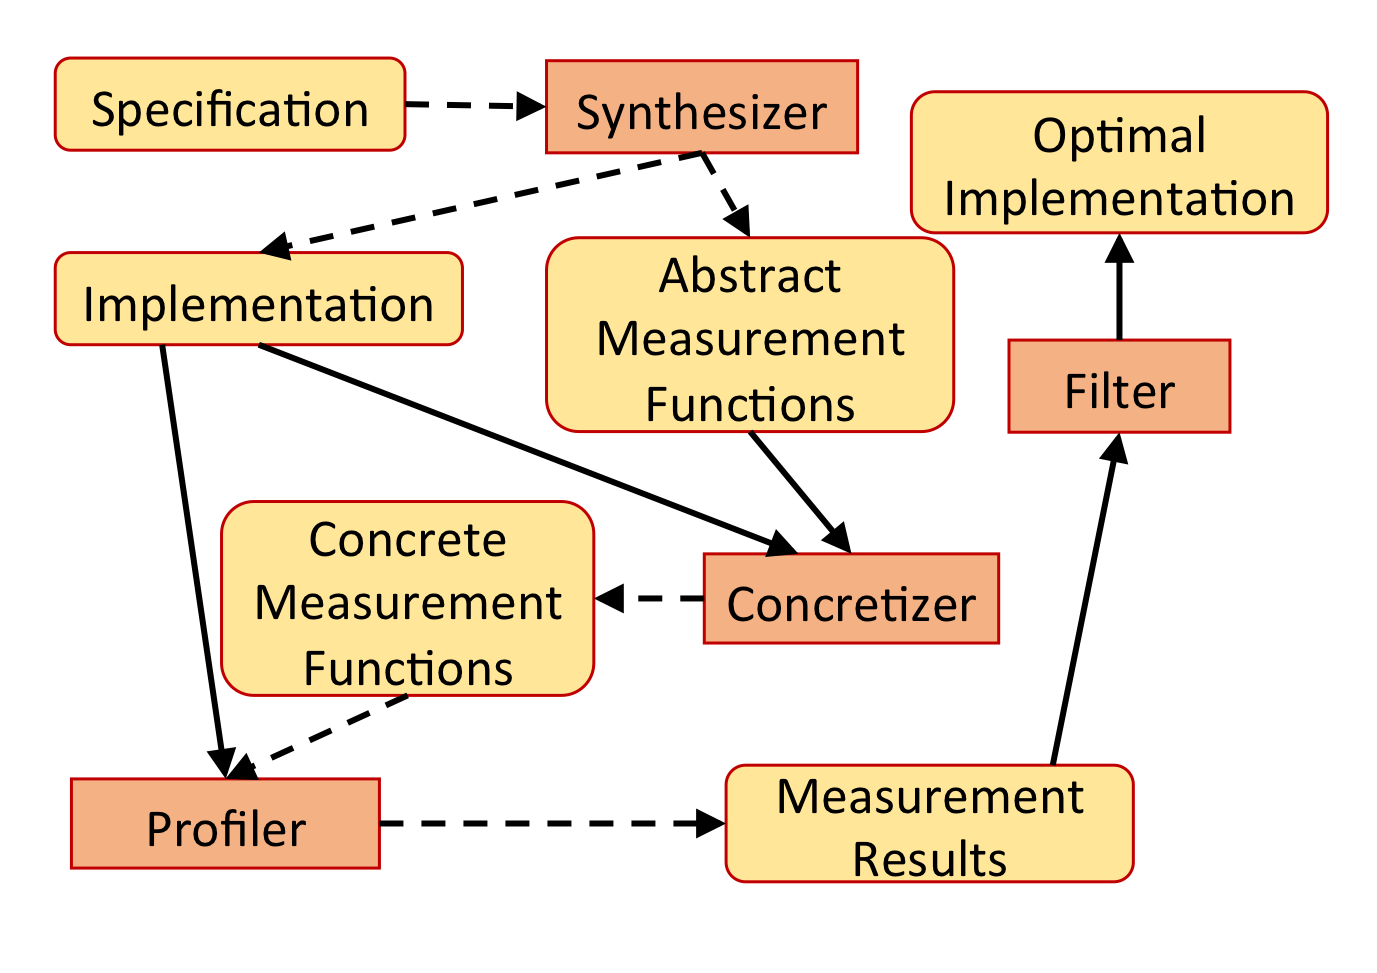
\includegraphics[width=0.9\textwidth]{img/structure}
\caption{Framework Data Flow}
\label{fig:framework_structure}
\end{figure}


We have exploited the idea of using typeclasses to capture general families of mathematical structures by having our typeclass-based specification define the {\em family} of Astronaut instances, including dimensions of variation, shared operations, and invariants common to all family members. %Ordinary functional programming languages do not support the expression of logical invariants in the declarative, expressive, higher-order constructive logical style that Coq supports. To our knowledge, the interesting but at best only modestly deep observation that Coq typeclasses can be used to specify program families, including structural and behavioral invariants, is novel.
Typeclasses in Coq are useful for specifying interrelated {\em families} of mathematical structures, including carrier sets, operations, and invariants, as well as for specifying instances of these structures. An example of interrelated families of structure from abstract algebra include monoids, groups, and fields (each of which enriches the previous one).

The structure of our framework is shown in more detail in Figure~\ref{fig:framework_structure}. It takes user defined specifications as inputs. The synthesizer then synthesizes a set of implementation and associated test loads. Next, the measurement function dynamically analyzes each implementation with associated test loads to get a set of measurement results for each solution point. At last, the filter picks the set of (Pareto-)optimal solutions based on the measurement results.


\subsection{Astronaut Typeclass}
Astronaut is the most abstract, least structured typeclass in our hierarchy. It expresses the functionality of a broad family of tradespace analysis tools at a high level of abstraction. The code fragments in Listing 1 presents the hierarchy of abstract algebraic structures that we formalized as Coq typeclasses. Each typeclass (\textsf{Set} in the code) characterizes a class of possible instances. Each class represents a type, values of the type, operations on the type, and laws constraining the behaviors of the operations. It has four types: (1) type of input specification (e.g., a UML class diagram); (2) type of derived implementation (e.g., SQL schema); (3) type of a set of property measurement functions (e.g., space performance measurement); and (4) type of measurement results (e.g., database size in megabytes). Values have to be provided when instantiating Astronaut typeclass. %The specification hardwires what amounts to a batch-sequential map-reduce structure, with exhaustive synthesis completed before map-reduce evaluation begins.

\begin{figure}
\vspace{1cm}
\begin{lstlisting}[
mathescape,
basicstyle=\footnotesize\sffamily, %\scriptsize,
keywordstyle=\color{blue}\bfseries,
commentstyle=\color{red},
stringstyle=\ttfamily,
numbers=left,					% where to put the line-numbers
numberstyle=\scriptsize,			%\tiny,      
frame=tb,
xleftmargin=1.5em,
escapeinside={(*@}{@*)},	
morekeywords={set,Set,Class,list,forall,set}
escapeinside={(*@}{@*)},
showstringspaces=false,
label={lst:tradespace_typeclass},
captionpos=b,
caption={Astronaut Typeclass Coq specification, which defines the most abstracted framework structure. It takes a specification as input, and outputs a set of implementations and measurement results.}]
Class Astronaut := {
  SpecType: Set
; ImplType: Set
; MeasureFuncSetType: Set
; MeasureResultSetType: Set
; synthesize : SpecType ->
    list(ImplType $\ensuremath{\times}$ MeasurFuncSetType)
; mapReduce: list (ImplType $\ensuremath{\times}$
    	MeasureFunctSetType) ->
    list (ImplType $\ensuremath{\times}$ MeasureResultSetType)
; astronaut (spec: SpecType):
    list (ImplType $\ensuremath{\times}$ MeasureResultSetType) :=
    map mapReduce (synthesize spec)
}.
\end{lstlisting}
 \end{figure}

The {\em synthesize} component is a function that maps a specification to lists of $<Implementation, MeasurementFunction>$ pairs. The measurement functions provide performance comparisons of variant implementations. The {\em mapReduce} component is a function that takes a list of $<Implementation, MeasurementFunction>$ pairs, and returns a list of $<Implementation, MeasurementResult>$ pairs. The {\em astronaut} function calls the {\em map} function to map the measurement functions over the output of the synthesize function (a list of $<Implementation, MeasurementFucntion>$ pairs). Implementations of these functions are required when the typeclass is instantiated.

%\newpage
\subsection{Tradespace Typeclass}
The Astronaut typeclass\footnote{Research artifacts and the complete model for \@approach, including all specifications, are available at http://chongtang.github.io/Astronaut/} (Listing 1) captures a very general notion of tradespace analysis, and nicely illustrates some of the aspects of our approach, but it provides too few details for implementing a tradespace analysis tool. We introduce a new tradespace typeclass to enrich the Astronaut typeclass to provide a finer-grained implementation architecture for tradespace analyzers.

\begin{figure}[t!]
\vspace{0.5cm}
\centering
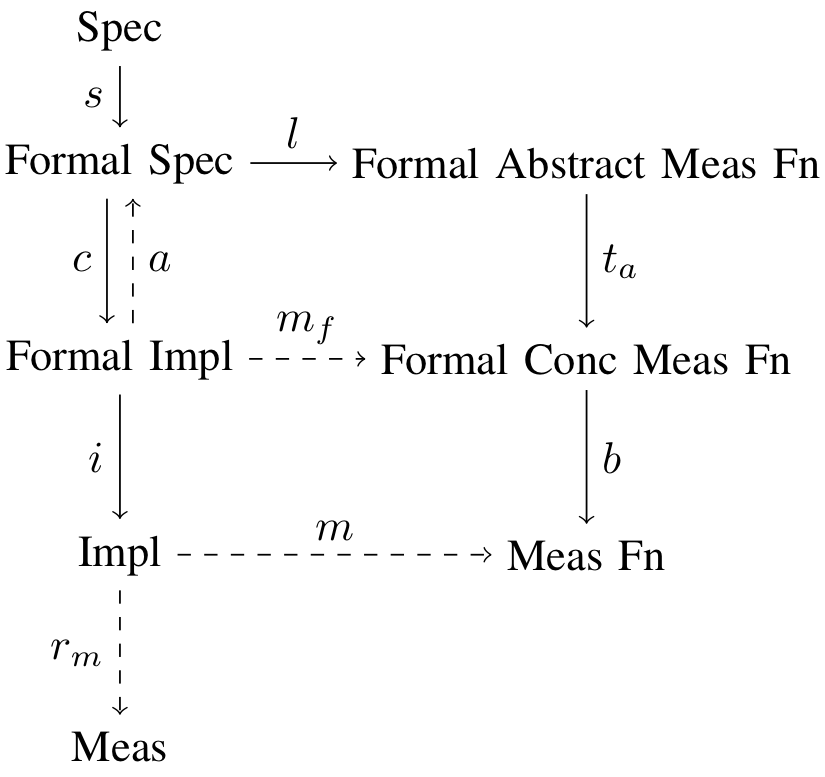
\includegraphics[width=0.8\textwidth]{img/tradespace_model.png}
\caption{Tradespace typeclass model}
\label{fig:tradespace_model}
\end{figure}

Listing~\ref{lst:tradespace_typeclass} partially presents Tradespace typeclass Coq specification. 
The first two lines state that the {\em Tradespace} class extends (is coercible to) the Astronaut and ParetoFront typeclasses. The latter provides structure for computing Pareto fronts of sets of vector-valued objects. The following four components (lines 5--8) provide for parameterization of typeclass instances with respect to the key additional types of the implementation framework. Following the declarations of these type-valued parameters, lines 10--21 specify the signatures of the mapping functions required to instantiate the Tradespace typeclass.
%, as the functions ($c, a, l, t_a, a, s, i, b$) illustrated in Figure~\ref{fig:tradespace_model}. 

The diagram shown in Figure~\ref{fig:tradespace_model} graphically depicts the structure of the Tradespace typeclass.
The concretization function (\textsf{cFunction}) maps the formal specification to a set of formal representations of implementations (\textsf{FmImplType}). The function abstraction (\textsf{aFunction}) explains how each implementation represents and satisfies its specification. The load function (\textsf{lFunction}) maps the same formal specification to a set of abstract measurement functions (\textsf{FmAbsMeasureFuncSetType}) that will be used to produce concrete measurement function (\textsf{FmConcMeasureFuncSetType}) to measure the properties of implementations. The function \textsf{tFunction} is a conceptual function serves our explanation here and doesn't require implementation. It specializes the abstract measurement functions to the particular interfaces exposed by variant implementations. This function uses the abstraction function \textsf{aFunction} to do its work. The result of this process is another conceptual function/relation, as indicated by $m_f$ in Figure~\ref{fig:tradespace_model}, that associates a vector of implementation specific measurement function(s) to each implementation. 

The function \textsf{sFunction} translates a user given specification to an internal formal specification that can be solved by \textsf{cFunction}. The function \textsf{iFunction} parses the formal/internal representation of implementations to usable forms: e.g., Alloy solutions to SQL schemas. The function \textsf{bFunction} similarly parses formal/internal representation of measurement functions to useful forms: e.g., to objects that run actual SQL scripts against actual databases. The final tradespace analysis result is the relation $r_m$ in Figure~\ref{fig:tradespace_model} that associates implementations with their corresponding property measurement vectors.

The final three components (lines 23--30) specify laws that the other components of the typeclass must follow. In a nutshell, these laws state that the abstraction function, $a$, must invert the concretization function, $c$, and that the two paths from specification to measurements must yield the same results. Constructing an instance of the typeclass requires proofs of these propositions for the given function and data type parameter values.

\begin{figure}
\vspace{0.5cm}
\begin{lstlisting}[
mathescape,
basicstyle=\footnotesize\sffamily, %\scriptsize,
keywordstyle=\color{blue}\bfseries,
commentstyle=\color{red},
stringstyle=\ttfamily,
numbers=left,					% where to put the line-numbers
numberstyle=\scriptsize,			%\tiny,      
frame=tb,
xleftmargin=1.5em,
escapeinside={(*@}{@*)},	
morekeywords={set,Set,Class,list,forall,set}
escapeinside={(*@}{@*)},
showstringspaces=false,
label={lst:tradespace_typeclass},
captionpos=b,
caption={Tradespace Typeclass Coq specification. It captures the internal structure of our framework.}]
Class Tradespace := {
  tm_Astronaut :> Astronaut
; tm_ParetoFront :> ParetoFront
(*@\textcolor{comments}{\textbf{(* Internal, Formal-Spec-based types *)}} @*)
; FmSpecType: Set
; FmImplType: Set
; FmAbsMeasureFuncSetType: Set
; FmConcMeasureFuncSetType: Set
(*@\textcolor{comments}{\textbf{(* Internal, Formal-Spec-based functions *)}} @*)
; cFunction: FmSpecType -> list FmImplType
; aFunction: FmImplType -> FmSpecType
; lFunction: FmSpecType ->
             FmAbsMeasureFuncSetType
; tFunction: FmAbsMeasureFuncSetType ->
             list ImplType ->
             list FmConcMeasureFuncSetType
(*@\textcolor{comments}{\textbf{(* map to and from Formal-Spec-based form *)}} @*)             
; sFunction: SpecType -> FmSpecType
; iFunction: FmImplType -> ImplType
; bFunction: FmConcMeasureFuncSetType ->
             MeasureFuncSetType
(*@\textcolor{comments}{\textbf{(* Laws *)}} @*)             
; aInvertsC: forall (spec: FmSpecType)
             (fImpl: FmImplType),
             In fImpl (cFunction spec) ->
             (spec = aFunction fImpl)
(*@\textcolor{comments}{\textbf{(* See code repo, omission on purpose. *)}} @*)                          
; implLineLaw: ...
(*@\textcolor{comments}{\textbf{(* See code repo, omission on purpose. *)}} @*)                          
; testLoadsLineLaw: ...
}.
\end{lstlisting}
\end{figure}



\section{Framework Instantiation}
\label{tool_implementation}
Framework users need to provide domain-specific types for the nodes in Figure~\ref{fig:tradespace_model} and domain-specific function implementations for the solid arcs. The other dashed-line mappings are implicit or automatically computed. %Our main tool implementation effort was in producing Scala types and functions exactly in correspondence with Figure~\ref{fig:tradespace_model}, as required by the Coq specification. 
This section describes how we instantiate our framework to create an automation tool in the context of the ORM domain. 

To instantiate an automated tool based on the framework for ORM tradespace analysis, we defined a $DBFormalSpec$ class as an actual parameter for the $Formal Spec$ slot in this architecture (cf.~Fig.~\ref{fig:tradespace_model}). Concretely, it is a wrapper around a file containing Alloy specification of an object model. Similarly, we created a $DBImplementation$ class that wraps a file containing a MySQL schema definition, as a parameter for the $Impl$ in Figure~\ref{fig:tradespace_model}. Our implementation of the function $c$ realizes our Alloy-based approach to synthesize database schemas from object models. Our other ORM-specific values are similar in their structure: classes (Scala types) wrap representation details and function implementations such that they encapsulate details of computations of the various mappings required to implement our tradespace analysis approach. We also implemented $mapReduce$ function in Astronaut typeclass using Spark library for Scala. When the tool actually runs, it sends measurement jobs to a pre-configured Spark cluster.

We then provided several parameter values to instantiate the framework. The components include: 1) An Alloy-based ORM domain specification language; 2) an Alloy-based synthesizer to generate candidate designs and test loads (INSERT and SELECT SQL scripts) to be executed to dynamically analyze database designs; 3) two kinds of measurement functions ({\em Time} and {\em Space} measurement functions) to measure time and space tradeoffs; 4) a triple of population time, retrieval time, and space consumption as a group of analysis results; and 5) a Pareto-optimal filter to filter out non-Pareto-optimal designs.

Our instance for ORM analysis of this framework is produced with the following parameters.
\begin{itemize}
\setlength{\itemsep}{0pt}
\setlength{\parskip}{0pt}
\item \textsf{SpecType}: Object models in formal Alloy-based notation
\item \textsf{ImplType}: SQL schema
\item \textsf{MeasureFuncSetType}: an instrumented test harness for profiled execution of synthesized SQL scripts
\item \textsf{MeasureResultSetType}: a tuple of time and space performance measures from instrumented benchmark execution
\item \textsf{synthesize}: given an object model, produce a list of SQL schema and SQL script pairs (INSERT and SELECT statements) 
\item \textsf{mapReduce}: run a profiled SQL script on a database with the given schema in map-reduce style %and return the schema measurement pair
\item \textsf{sFunction}: An identity function (since the Specification Type in our case is already a formal object model)
\item \textsf{cFunction}: Alloy based analyzer that synthesizes an object model to a set of database designs in the form of database creation scripts
\item \textsf{aFunction}: A function that returns the mapping information in each database design
\item \textsf{lFunction}: A generator that creates formal abstract measurement functions from an object model
\item \textsf{tFunction}: A concrete formal measurement function specializer that mapping a formal abstract measurement function to a set of concrete measurement functions based on mapping information of each designs
\item \textsf{iFunction}: A parser that parses the database schema embedded in Alloy solution (XML files) to SQL database initial script
\item \textsf{bFunction}: An identity function (the formal concrete measurement function in our case is already INSERT and SELECT SQL statements)
\end{itemize}

%There are two outcomes we value from the experiments: 1) reduction in the human cost of tradespace analysis, 2) the potential for improvement in design results relative to those produced by commonly used methods. We thus present our experimental setup and results in rest paragraphs.
 
%\section{Tradespace Synthesis from Relational Logic}
 


%%%%%%%%%%%%%%%%%%%%%%%%%%%%%%%%%%%%%%%%%%%%%%%%%%%%%
%\section{Parallelization of Solution Points Analyses} 
\section{Parallelization Reasoning} %%Parallel Analysis of Solutions}
\label{parallelization}

Even simple specifications could map into a vast number of solutions in the design space. The combination of ample computing capacity and our ability to synthesize immense solution spaces for given specifications suggests that we measure properties and tradeoffs of actual running systems in the spirit of what Cadar et al. called multiplicity computing~\cite{cadar_multiplicity_2010}, with the goal of producing new speed-ups in tradeoff analysis of real-world software systems.

%The combination of ample computing capacity and our ability to split a given, complex specification into independently analyzable slices suggests that we separately compute the solution spaces of various slices, and incremen- tally merge them, with the goal of producing new speed-ups in bounded verification of large-scale systems.

%Even a simple specification could maps into a large number of solutions in the design space. Suppose the number of unspecified properties of a specification is $n$ (cf.~Section~\ref{problem}), the number of solutions for such a specification could be as large as $2^n$ due to the complex interactions among those properties. All these solutions consist a property vector with $n$ dimensions of values. It is hard to generate such a large space, as well as to measure every solution in the space. In the filed of program synthesis, researchers usually use a SAT solver to exhaustively generate every possible points. Although it is still impossible to generate the tradeoff space for arbitrary large size of specification, it's plausible to solve a middle size specification thanks to the advance in SAT solver research. However, how to evaluate all solutions so that we pick the one or few that have desired properties tradeoff is something hard to proceed.

%Researchers have show that static analysis does not always work in evaluating the practical performance of a system~\cite{ICSE_2014_paper}. It's understandable because static analysis lose the information of dynamic running environment, as well as the dynamic size of input that a system could meet in production environment. Although there are some guide techniques that can somehow direct the space search procedure to find a desired solution quickly \textbf{Hamid, is there any citations here. Maybe Westley Weimer's GenProg paper?}, there is no guarantee that these techniques can the right one.

%A better solution is to dynamically measure the performance of all solutions in the tradespace, and then select the corresponding program according to the measurement results. However, due to the large number of solutions and their large size of test loads, it is not possible to evaluate all of them in an acceptable time. In this project, we present a method to parallelize the measurement process on top of Spark.

%Not all phases in a synthesis+measurement task can be parallelized. Given a specification, the whole process of program synthesis and measurement has multiple phases: 1) synthesize formal program; 2) synthesize abstract test load; 3) concretize program; 4) concretize test load; 5) measure the performance of a program. Phase 1 and 2 need a SAT solver to solve the specification. As to our knowledge, there is no parallelization SAT solver so far. Thus phase 1 and 2 can only be done in a single machine. In this project, we parallelize phase 3, 4, and 5.


%Recall that tradeoff analysis using our approach consists of three steps: (1) Solution space and test loads are synthesized from formal specifications. (2) The synthesized solutions and test loads are transformed into concrete formats, e.g., here Alloy models are concretized into database schemas and corresponding test loads.  (3) Dynamic analysis of synthesized tradespaces by profiling performance of each database solution under its corresponding schema-specific test loads. In this section, we focus on steps 2 and 3 that can significantly benefit from parallelizing the process.  

Recall that tradeoff analysis using our approach consists of three steps: (1) Solution space and abstract measurement functions are synthesized from formal specifications. (2) The synthesized implementations and abstract measurement functions are transformed into concrete formats, e.g., here formal models are concretized into database schemas and corresponding test loads. (3) Synthesized solution spaces are dynamically analyzed by profiling performance of each solution under its corresponding structure-specific measurement function. In this section, we focus on steps 2 and 3 that can significantly benefit from parallelizing the process.

\newcommand\floor[1]{\lfloor#1\rfloor}
\newcommand\ceil[1]{\lceil#1\rceil}
%The step (1) is done on the master node, and step (2) and (3) are done on multiple worker nodes. In step (1), 
%Astronaut executes the \emph{synthesize} function to generate a set of solution implementations and the abstract measurement functions. In a tradeoff space, there are multiple implementations and one set of abstract measurement functions for all implementations. In step (2), Astronaut distributively sends out the generated implementations to all worker nodes, along with one copy of the abstract measurement functions. When it sends out implementations, Astronaut tries to spread the workload of each worker node equally. For example, if there are $m$ generated implementations and $n$ worker nodes, then each worker will be assigned about $\floor{\frac{m}{n}}$ implementations to evaluate. In step (3), all workers will run in parallel to execute the concrete measurement functions and profile performance of each assigned implementation.

%Algorithm~\ref{alg:para_eval} shows how a worker node concretizes the abstract measurement functions based on the abstraction function generated by \emph{synthesize} function in step (1). The inputs of this concretize+dynamic evaluation logic include a implementation to be evaluated, a set of the abstract measurement functions, and a abstraction function which contains information of how each component of the given implementation is mapped from the specification. Such information will be used to guide the process of concrete measurement functions generation. The abstract measurement functions in our case is a Java HashMap object that contains all test data. The concrete measurement functions are \emph{Insert} and \emph{Select} SQL statements that will be executed to profile database schemas.


\renewcommand{\algorithmicrequire}{\textbf{Input:}}
\renewcommand{\algorithmicensure}{\textbf{Output:}}

%\begin{figure}

\begin{algorithm}[tb]
%\vspace{0.5cm}
\caption{Profiling a given design solution in a worker node.} %A worker node generates concrete measurement functions for an implementation, and then evaluates it.}
\label{alg:para_eval}
\begin{algorithmic}[1]
\REQUIRE $i$: Formal Impl, \textcolor{comments}{\textbf{// design to be analyzed}} \\
 		 $f_a$: AbstractionFn, \textcolor{comments}{\textbf{// abstraction function}} \\
		$M_a$: List<AbstractMeasFn> \\\textcolor{comments}{\textbf{// abstract measurement functions}} \\ 
\ENSURE p: Result \textcolor{comments}{\textbf{// profiling evaluation results}}

\STATE $M_c = new List()$ \textcolor{comments}{\textbf{// concrete measurement functions}} \\ 
\FOR{$m_a \in M_a$}
	\STATE $m_c \gets generateConcreteMeasure(m_a, f_a, f)$
	\STATE $M_c.add(m_c)$
\ENDFOR

\STATE $profResults \gets new List()$
\FOR{$m_c$ in $M_c$}
	\FOR{$i$ in $[1:3]$}
		\STATE $result \gets runMeasureFunction(i, m_c)$
		\STATE $profResults.add(result)$
	\ENDFOR
\ENDFOR
\STATE $p \gets average(profResults)$
\RETURN $p$
\end{algorithmic}
\end{algorithm}
%\end{figure}

Similar to a conventional cluster computing paradigm, \@approach's approach for parallelization  consists of a large number of worker machines managed by a master node referred to as the cluster manager.
Once \@approach's cluster manager deploys a synthesized solution to a worker machine,
it runs to profile the performance of the given design solution in parallel with other worker machines.

Algorithm 1 outlines the process of profiling a given design solution as realized in a worker node. 
It takes as input (1) a design solution to be analyzed, $i$, (2) its associated abstraction function, $f_a$, that explains how the given design solution instantiates its abstract specification, and (3) a vector of measurement functions, which are essentially abstract test loads automatically generated from the specification and need to be concretized for the given design solution. 

The logic of the algorithm is as follows. For each abstract measurement function, $m_a \in M_a$, generate concrete measurement functions, or test loads, that meet the particular structure of the given design solution, $i$. In doing so, $generateConcreteMeasure$ relies on the abstraction function that relates the design solution back to the abstract specification from which input measurement function, or abstract test load, is derived, and that from these abstraction functions it derives functions for concretizing  the given abstract loads. After the measurement functions are generated for the given design, run them to profile its performance.

%Lines 1-5 generates concrete measurement functions for the given implementation. The abstraction function helps the concretization function in line 3 to generate concrete measurement functions that meet the particular structure of the given implementation, so that these functions can be executed successfully. After the measurement functions are generated, line 6-12 run them to profile the given implementation. Line 9 is where the actually dynamic profiling happens. We record the profiling results when we run the test loads. For example, when we run \emph{Insert} statements, we record the population time. After that, we check the space consumption of all data. When we run \emph{Select} statements, we record the data retrieval time. Each set of test loads will be executed 3 times, and the final profiling result is the average of 3 recorded results. If there is an error happens so that the whole process cannot be finished successfully. The master will be notified and it will send the job to another worker.

%The whole logic is executed in distributed manner by worker machines. Compare to the single machine scenario, this parallel approach speeds up the concrete measurement function generation and the dynamic profiling process, which are the most space-consuming and time-consuming step respectively in this whole approach. A single machine usually doesn't have enough resource to support such large space and computing power requirements.

%%%%%%%%%%%%%%%%%%%%%%%%%%%%%%%%%%%%%%%%%%%%%%%%%%%%%%

\begin{comment}
\section{Prior Work}

The idea of design space exploration and tradeoff analysis is decades old, and the scientific and engineering literature and technology base in this area are extensive. A survey is beyond the scope of this work. This section further summarizes the relevant prior work on which this paper builds directly, namely that of Bagheri et al. 

Bagheri et al. developed RLTA, as realized in Trademaker, to determine whether relational logic model finders, such as Alloy, could be used for design synthesis and tradeoff analysis. Their approach is rooted in the following elements. 

First, specifications are written in domain-specific system specification languages (DSSLs) embedded in a relational logic. For example, Bagheri et al. developed a the Alloy-OM DSSL for specifying object-oriented data models. Alloy-OM is implemented as a set of ORM-specific Alloy signatures, which the user of Alloy-OM then extends to specify a particular object model.

Second, the non-deterministic semantics of such DSSLs are also expressed (one time only) in relational logic. These semantics express what it means for a design to satisfy a specification under the given semantics. That the semantics are non-deterministic means that in general there are many specification-satisfying designs. The semantics of Alloy-OM are defined in Alloy. They define a broad range of specification-satisfying (valid) strategies for mapping given object models to (Alloy encodings of) SQL relational database schemas. 

Third, RLTA uses general-purpose relational logic model finders to enumerate design models that satisfy the relational logic formula obtained by conjoining application-specific specifications with the specification language semantics. The result is an enumeration of (relational logic models of) the designs in the design space of the given specification. For example, Trademaker uses Alloy to exhaustive enumerate (Alloy encodings of) SQL schemas corresponding to object models specified in Alloy-OM. 

Fourth, Trademaker automatically applies {\em property prediction functions} (PPFs) to (Alloy encodings of) design models to predict their system properties. Bagheri et al. demonstrated the application of a previously published set of {\em static} PPFs to (Alloy representations of) design models. These functions took SQL database schemas as inputs and produced measures that were purported to roughly predict runtime performance characteristics for reads and writes as well as file size (space) performance, among other properties.

Trademaker automated this process, ran as a web-based tool, filtered and presented the results in useful forms (e.g., eliding results for strictly sub-optimal designs), and unparsed engineer-selected designs into useful forms. Trademaker would enumerate designs, apply PPFs to each, gather the results, classify the results into clusters, select a representative from each cluster, discard strictly suboptimal results, present the rest to the engineer, allow the engineer to pick a preferred solution, and finally deliver the result as an instantiated SQL script, unparsed from the corresponding relational logic design model, to create a MySQL database with the selected schema.

As noted in the introduction, this paper makes three novel contributions beyond the prior work of Bagheri et al. 
\begin{itemize}
\item Bagheri et al. had never previously tested the hypothesis that RLTA finds better designs than people are likely to find using standard (default) methods. This is a major hole in the earlier work, which this paper fills.
\item Trademaker was narrowly specialized for ORM and did not support {\em exhaustive, dynamic tradespace analysis.} Astronaut is a general-purpose framework for exhaustive, dynamic tradespace analysis, t	ested by its use on the experiments reported herein.
\item Previous work presented a quasi-mathematical sketch of the computational architecture of Trademaker. This paper presents a formal, mechanically checked theory of exhaustive, dynamic RLTA, from which Astronaut code was synthesized by Coq extraction.
\end{itemize}

%%%%%%%%%%%%%%%%%%%%%%%%%
%%%%%%%%%%%%%%%%%%%%%%%%%
%%%%%%%%%%%%%%%%%%%%%%%%%

\section{Roadmap}

The remaining sections of this paper are organized as follows. First we present our experiments and evidence in support of the hypothesis that RLTA can find designs that are strikingly better that those produced by commonly used (default) tools. Second, we present the design and our evaluation of the Astronaut tool. Our two main claims for Astronaut are that it (1) unsurprisingly vastly reduces the human effort required to dynamically profile exhaustively enumerated design spaces compared to the manual approach previously taken by Bagheri et al.; and (2) that it does provide its user with a general framework, supporting specialization to particular domains (here ORM) by extension of abstract OO framework base classes. Third, we provide an overview of our Coq specification. Fourth, we discuss our results and put them in a broader context. Fifth, we discuss other related work. Finally, we conclude.

\end{comment}

%%%%%%%%%%%%%%%%%%%%%%%%%
%%%%%%%%%%%%%%%%%%%%%%%%%
%%%%%%%%%%%%%%%%%%%%%%%%%

\section{Experimental Evaluation}
%\section{Experimental Evaluation}
\label{evaluation}
%This section describes how we use the tool instantiated from the framework to carry out database schema design and tradespace analysis. More importantly, we discuss the result design of synthesis + tradespace analysis, and the comparison between the result design with two other commonly used tools that built in Django and Ruby on Rails.   


%To test the capability of our theory and framework to support meaningful tradeoff analysis, as we have stated, we rebuilt our previous, ad hoc tradespace analysis tool to instantiate this theoretical framework.

To assess the effectiveness of our theory and framework in supporting tradeoff analysis, we have conducted an experimental evaluation that addresses the following research questions:
%We formulate, test, and provide experimental data in support of three driving hypotheses:

%As an experimental test of our approach to specification-driven, automated dynamic analysis of non-functional property tradeoffs across design spaces, we apply the approach to test the validity of the static predictors of database performance. 
%In this case, a further question arises: how to optimize dynamic analyses. We were thus led to formulate three driving hypotheses for the research reported in the rest of this paper:
%This paper formulates, tests, and provides experimental data in support of three driving hypotheses


\begin{itemize}
%1) how the approach works compare to industrial tools
%2) How much achievement one can gain through using the schemas generated by tradeoff analysis
%3) How well the approach works compare to state-of-the-art
%\item \textbf{RQ1.} Does \@approach's tradespace analysis enable production of designs that are overlooked by widely-used ORM tools? %that rely on single-point strategy?
%\item \textbf{RQ1.} Does \@approach tradespace analysis enable production of designs that are significantly better than those produced by widely-used ORM tools? %yet overlooked by such tools?
\item \textbf{RQ1.} Does \@approach tradespace analysis enable production of Pareto-optimal designs that are entirely overlooked by widely-used, industrial ORM tools? 
\item \textbf{RQ2.} How well does \@approach perform? What is the performance improvement achieved by \@approach's designs compared to those produced by industrial frameworks? 
%\item \textbf{RQ1.} How well does \@approach perform compared to widely-used ORM tools? %Does \@approach produce results than are significantly better than those produced produced by widely-used ORM tools?
\item \textbf{RQ3.} What is the overhead of \@approach in conducting tradespace analysis? 



%\item \textbf{RQ2.} How well does \@approach perform? What is the performance improvement achieved by \@approach's designs produced through tradespace analysis compared to designs produced by industrial frameworks?
%\item \textbf{RQ2.} How well does \@approach perform? What is the performance improvement achieved by \@approach's designs compared to those produced by industrial frameworks? 
\end{itemize}



This section summarizes the design and execution of our experiment, the data we collected, its interpretation, and our results. %, which include novel findings regarding these metrics.



\subsection{Experimental Objects}

Our experimental subjects are selected from different sources and of a variety of different domains, ranging from our research lab projects to applications adopted from the database literature and open- source software communities. 

The first is the object model of an E-commerce system adopted from Lau and Czarnecki~\cite{sean_quan_lau_domain_2006}. It represents a common architecture for open-source and commercial E-commerce systems. It has 15 classes connected by 9 associations with 7 inheritance relationships. The second and third object models are for systems we are developing in our lab. Decider is another system to support design space exploration. Its object model has 10 Classes, 11 Associations, and 5 inheritance relationships. The third object model is for the CSOS system, a  cyber-social operating system meant to help coordinate people and tasks. In scale, it has 14 Classes, 4 Associations, and 6 inheritance relationships.  
The fourth object model is the object model of a documents sharing application called Flagship Docs built with Ruby on Rails at Rensselaer Polytech \cite{FlagshipDocs4}. It has 6 classes connected by 8 associations with no inheritance relationships. We also analyzed an extended version of our customer-order example~\cite{trademaker}.
 

%On the one hand, all these subjects are simple and easy to abstract the database model. On the other hand, they are complicated enough to contains multiple relationships among objects. 
The selected experimental subjects are representatives of large classes of useful applications at a scale matched to the state-of-the-art synthesis techniques. Their databases have multiple tables, and several relationships among these tables. There are multiple ownership relationships among these tables, which induce many possible choices of object-model to relational schema mappings.

 

%\newpage
\subsection{Experimental Setup and Data Collection}

%We followed several steps to address the research questions. First, we wrote database specifications using Django, Rails, and the object-modelling language developed by Bagheri et al.~\cite{trademaker}, for each one of the five systems. Second, we synthesized schemas from five object models written in the modelling language along with SQL $INSERT$ and $SELECT$ commands for dynamic analysis. Third, we created databases with synthesized schemas and running the test loads to each one of them. While running the test SQL statements, we collected time consumed by each database, and the space consumption of each database after the execution of all $INSERT$ statements. We also collected the time and space consumption data for the database schemas produced by Django and Rails. %to determine their time and space performance.

We followed several steps to address the research questions. First, we wrote database specifications using Django, Rails, and the object-modelling language developed by Bagheri et al.~\cite{trademaker}, for each one of the five systems.
%There are four basic operations on a database, often called CRUD: Create, Read, Update, Delete. 
We chose to focus on time and space performance of \emph{CREATE} and \emph{READ} transactions for dynamic analysis of target database performance. We wrote instrumentation code to return the desired time and space consumption data into the map-reduce computation. We used the \emph{mysql} client command to execute synthesized test loads, which our tool parses from internal Alloy representations into MySQL scripts. The first sets of statements were database structure creation scripts. Then \emph{insert} scripts were executed to populate each database with the test data generated in previous stages. The experimental data collected includes the time to run these commands as well as the space consumed by the databases. After populating the databases with test data, we executed \emph{READ} transactions, which are essentially collections of \emph{select} commands.  We ran each script three times to rule out other uncontrolled factors that might influence the data we collected. The evaluation results are a list of triples: insertion time, retrieval time, and space consumption. The final result reported in this paper is the average time and space performance.

%\begin{comment}

%\subsection{Data Analysis and Interpretation}
 

%What we really care about is the performance improvement produced by our approach. The improvements should be in two parts: 1) the performance improvement of Pareto-optimal database schemas synthesized by our technique, comparing to the performance of schemas produced by~{\em Ruby on Rails} and ~{\em Django}; 2) the improvement in analysis process that our automated analysis tool benefits comparing to manually conducted performance analysis.

%\end{comment}

%\subsection{Experimental Results}
%In this section, we present the experimental results about both our framework and the tradeoff space analysis.

\subsection{Astronaut vs. Industrial Platforms} %%Comparison with Widely-used Tools}
Figure~\ref{fig:analysis_result} depicts tradeoff analysis plots produced by \@approach.
It projects the results into 2-D tradeoff plots: Each plot presents tradeoff information in two of the three dimensions for one subject system. 
Each dot in the plots represents the analysis result of one schema. 
The hollow triangles that connected by a line are the Pareto-optimal designs in corresponding tradeoff space, exhibiting Pareto-optimal solutions in each plot. 
We also find out the two schemas produced by~{\em Rails} and ~{\em Django} from the synthesized schemas, by looking up the structure in SQL scripts. We then locate the analysis results of these two schemas, and mark them in the 2-D plots with different color and shapes. 
The hollow star is the design created by Django. The hollow diamond depicts the design generated by Rails.
One can easily distinguish the schemas from the other synthesized schemas, indicating where the {\em Rails} and {\em Django} generated schemas are fall in the tradespace in terms of the triple measures.


Consider the CSOS Insert-Space tradeoff plot (Row 2 and Column 2) as an example. It shows the tradeoff information of insertion time (in seconds) and space consumption (in megabytes). The two triangle depicts the Pareto front in these two dimensions. It could be just one triangle if there were only one design on the frontier. We can observe that although the schemas created by these tools are not same, their performances outcomes are close together. The most interesting point is that both of the generated schemas by these tools are far from the Pareto fronts. The same phenomena appear in other plots as well. 


The experimental data thus suggests that \@approach tradespace analysis enables production of Pareto-optimal designs that are entirely overlooked by widely-used, industrial ORM tools. 
 
%tradespace analysis enables production of database designs that significantly outperform those produced by industrial ORM synthesis tools, such as Rails and Django, yet are entirely overlooked by such widely-used, industrial tools.
 
\begin{figure*}[hbtp]
\centering
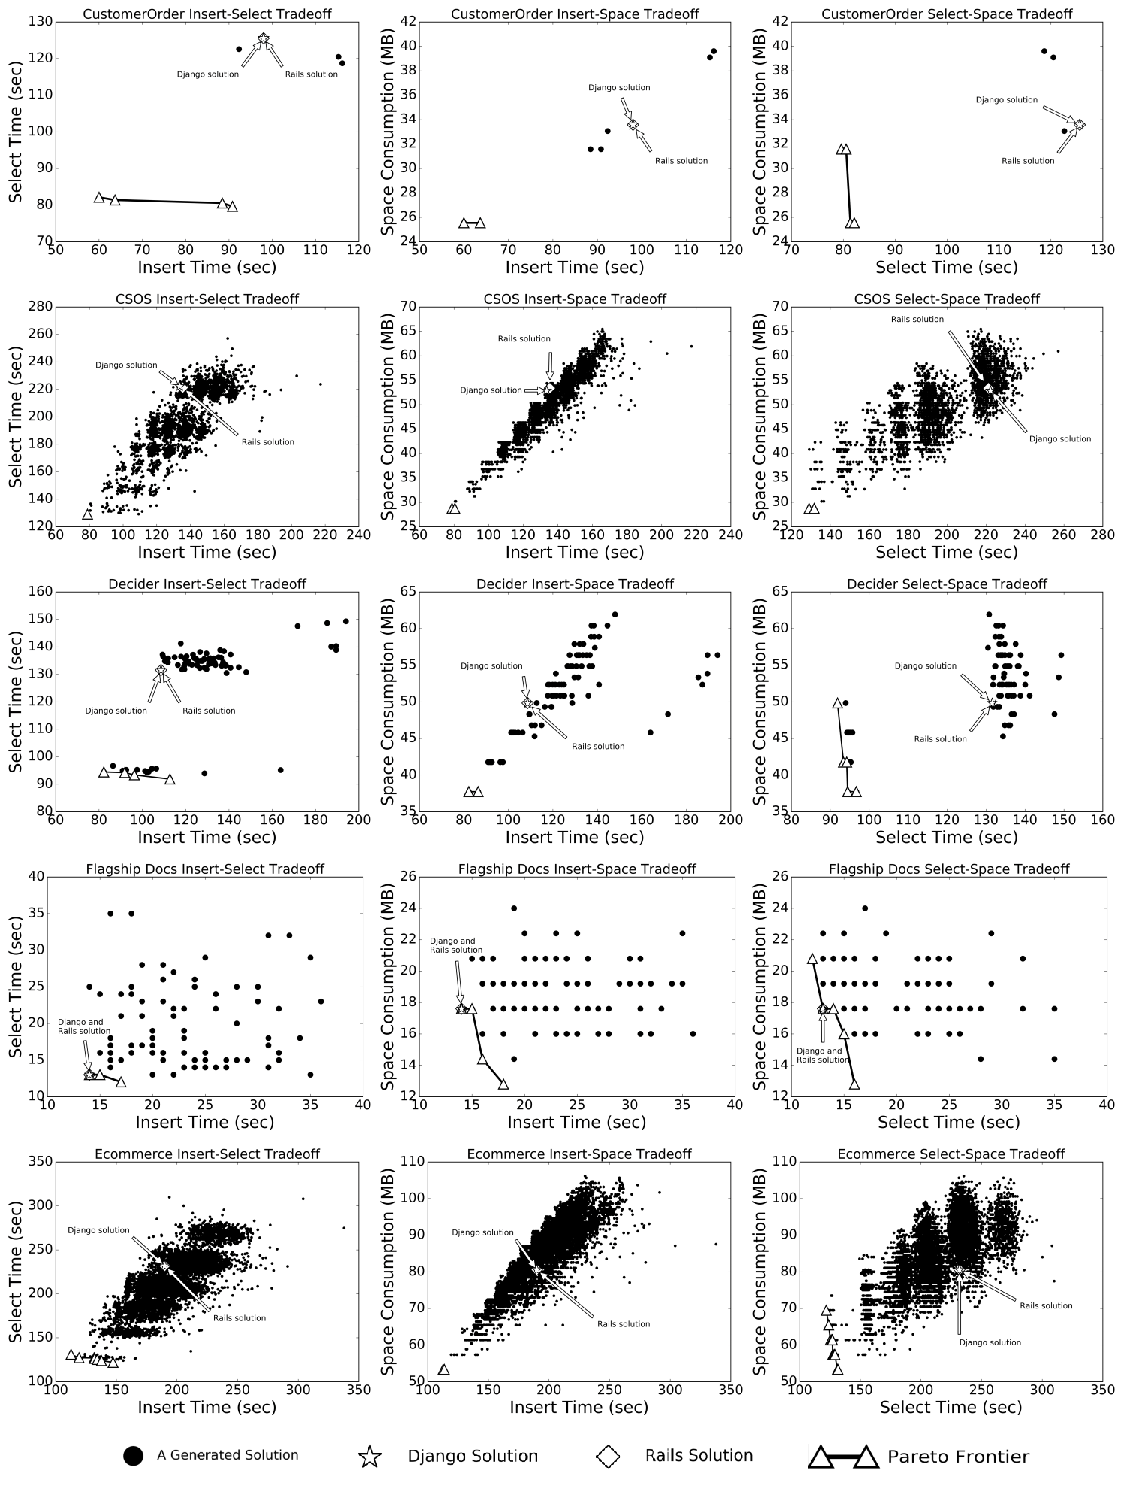
\includegraphics[width=\textwidth]{img/result_figure.pdf}
\vspace{-1cm}
\caption{Tradeoff analysis results; columns represent tradeoff diagrams across systems in two dimensions of Insert-Select, Insert-Space and Select-Space from left to right, respectively; each black dot represents performance of a synthesized database schema, and the star and diamond entries plot where the results of schema generated by Django and Ruby fall, respectively; both star and diamond entries are far from the Pareto fronts generated by \@approach.
}
\label{fig:analysis_result}
\end{figure*}


\subsection{Improvements in Practice} %Improvements Over Widely-used Tools}


%Our results support the hypothesis that our synthesis + tradespace exploration approach can produce significantly and strictly better designs than engineers produced using commonly used ORM tools. Our synthesize technique can generate better database schemas in terms of {\em Insert}, {\em Select}, and {\em Space Consumption} performance.

Table \ref{table:ts_imp_insert} presents the performance improvement in the insertion time by comparing a Pareto-optimal schema produced by \@approach to the performance of databases created by   Rails and Django ORM systems. The first line are the five experimental subjects. The second line is the insertion time consumed by the \@approach's designs. The third line is insertion time consumed by the {\em Rails} designs, and the forth line is insertion time consumed by {\em Django} designs. Finally, the last line represents the average performance improvement over {\em Rails} and {\em Django} designs across subject systems. %We compute the performance improvement by following formula: $$imp (percentage) = \frac{old-improved}{improved}*100$$ , in which $old$ is time performance of designs generated by {\em Rails} and {\em Django}, and {\em improved} is the time performance of Pareto-optimal designs.
Table~\ref{table:ts_imp_select} and table~\ref{table:ts_imp_space} similarly tabularize the performance improvement in the retrieval time and space consumption. %using the same formula as above.

From the experimental results, we can observe that the Pareto-optimal designs revealed by our analysis generally have much better performance in all dimensions: insertion times, retrieval times, and space consumption. Based on these analysis results, we conclude that our synthesis technique tends to perform better than commonly used tools, particularly, {\em Rails} and {\em Django}. Our synthesized designs have better performance, in three models: {\em CustomerOrder}, {\em CSOS}, {\em ECommerce}, and {\em Decider}, in all three dimensions. For the {\em Flagship Docs} model, {\em Rails} and {\em Django} produced designs equal to ours in performance. We have ascertained that the reason is that the {\em Flagship Docs} data model has no inheritance relationship, so all of the objects in the object model are mapped as an independent tables in synthesized database schemas.


\begin{table}[ht]
\begin{tabular}{@{}llllll@{}}
\hline
\hline
Subject & CO & CSOS & EComm & Decider & Flagship \\\cmidrule(r){1-6}
\@approach & 60.01 & 78.89 & 112.64 & 82.24 & 13.23 \\\cmidrule(r){1-6}
Rails & 97.99 & 133.61 & 189.93 & 108.62 & 13.23 \\\cmidrule(r){1-6}
Django & 97.99 & 135.41 & 189.93 & 108.62 & 13.23 \\%\cmidrule(r){1-6}
\toprule
\begin{tabular}[c]{@{}l@{}}Average\\Improvement\end{tabular} & 63.3\% & 70.5\% & 68.6\% & 32.1\% & 0\% \\%\cmidrule(r){1-6}
%{\color[HTML]{FE0000} \begin{tabular}[c]{@{}l@{}}IMP Over\\Rails\end{tabular}} & {\color[HTML]{FE0000} 63.3\%} & {\color[HTML]{FE0000} 69.4\%} & {\color[HTML]{FE0000} 68.6\%} & {\color[HTML]{FE0000} 32.1\%} & {\color[HTML]{FE0000} 0\%} \\\cmidrule(r){1-6}
%{\color[HTML]{FE0000} \begin{tabular}[c]{@{}l@{}}IMP Over\\Django\end{tabular}} & {\color[HTML]{FE0000} 63.3\%} & {\color[HTML]{FE0000} 71.6\%} & {\color[HTML]{FE0000} 68.6\%} & {\color[HTML]{FE0000} 32.1\%} & {\color[HTML]{FE0000} 0\%} \\
%\bottomrule
\hline
\hline
\end{tabular}
\caption{Insertion Performance (Seconds)}
\label{table:ts_imp_insert}
\end{table}

\begin{table}[ht]
\begin{tabular}{@{}llllll@{}}
%\toprule
\hline
\hline
Subject & CO & CSOS & EComm & Decider & Flagship \\\cmidrule(r){1-6}
\@approach & 82.12 & 129.10 & 131.09 & 94.46 & 14.03 \\\cmidrule(r){1-6}
Rails & 125.54 & 222.25 & 231.66 & 131.57 & 14.03 \\\cmidrule(r){1-6}
Django & 125.54 & 221.25 & 231.66 & 131.57 & 14.03 \\%\cmidrule(r){1-6}
\toprule
\begin{tabular}[c]{@{}l@{}}Average\\Improvement\end{tabular} & 52.8\% & 71.8\% & 76.7\% & 39.3\% & 0\% \\%\cmidrule(r){1-6}
%{\color[HTML]{FE0000} \begin{tabular}[c]{@{}l@{}}IMP Over\\Rails\end{tabular}} & {\color[HTML]{FE0000} 52.8\%} & {\color[HTML]{FE0000} 72.2\%} & {\color[HTML]{FE0000} 76.7\%} & {\color[HTML]{FE0000} 39.3\%} & {\color[HTML]{FE0000} 0\%} \\\cmidrule(r){1-6}
%{\color[HTML]{FE0000} \begin{tabular}[c]{@{}l@{}}IMP Over\\Django\end{tabular}} & {\color[HTML]{FE0000} 52.8\%} & {\color[HTML]{FE0000} 71.4\%} & {\color[HTML]{FE0000} 76.7\%} & {\color[HTML]{FE0000} 39.3\%} & {\color[HTML]{FE0000} 0\%} \\
%\bottomrule
\hline
\hline
\end{tabular}
\caption{Retrieval Performance (Seconds)}
\label{table:ts_imp_select}
\end{table}

\begin{table}[ht]
\begin{tabular}{@{}llllll@{}}
%\toprule
\hline
\hline
Subject & CO & CSOS & EComm & Decider & Flagship \\\cmidrule(r){1-6}
\@approach & 25.55 & 28.72 & 53.34 & 37.73 & 17.64 \\\cmidrule(r){1-6}
Rails & 33.58 & 52.86 & 80.56 & 49.83 & 17.64 \\\cmidrule(r){1-6}
Django & 33.58 & 53.36 & 80.56 & 49.83 & 17.64 \\%\cmidrule(r){1-6}
\toprule
\begin{tabular}[c]{@{}l@{}}Average\\Improvement\end{tabular} & 31.4\% & 85.0\% & 51\% & 32.1\% & 0\% \\%\cmidrule(r){1-6}
%{\color[HTML]{FE0000} \begin{tabular}[c]{@{}l@{}}IMP Over\\Rails\end{tabular}} & {\color[HTML]{FE0000} 31.4\%} & {\color[HTML]{FE0000} 84.1\%} & {\color[HTML]{FE0000} 51\%} & {\color[HTML]{FE0000} 32.1\%} & {\color[HTML]{FE0000} 0\%} \\\cmidrule(r){1-6}
%{\color[HTML]{FE0000} \begin{tabular}[c]{@{}l@{}}IMP Over\\Django\end{tabular}} & {\color[HTML]{FE0000} 31.4\%} & {\color[HTML]{FE0000} 85.9\%} & {\color[HTML]{FE0000} 51\%} & {\color[HTML]{FE0000} 32.1\%} & {\color[HTML]{FE0000} 0\%} \\
%\bottomrule
\hline
\hline
\end{tabular}
\caption{Space Consumption (MB)}
\label{table:ts_imp_space}
\end{table}

%%%%%%%%%%%%%%%%%%%%%%%%%
%%%%%%%%%%%%%%%%%%%%%%%%%
%%%%%%%%%%%%%%%%%%%%%%%%%

\subsection{Performance and Timing}

The final evaluation criteria are the performance benchmarks of tradespace analysis. To carry out the experiments,  we set up a 16-node Spark cluster as a back-end analysis platform. Each node has a 2-core AMD Opteron(tm) 242 CPU with kernel clock frequency of 1.5GHz, and 3 gigabytes of memory in total, where 1.9 gigabytes of memory is allocated to Spark. The worker nodes have MySQL server and client tools installed. 

Table~\ref{table:ts_time} shows the analysis time taken to produce tradespaces across subject systems. The first line are the five experimental subjects. The second line represents the size of tradespace for each subject system.  Finally, the last line shows the time required to automatically conduct the tradeoff analysis.

%The experimental results confirm that systematic dynamic tradespace analysis can find much better designs within plausibly practical time frames. 


%The results also confirm that an approach combin- ing static analysis and model checking is effective in compositional analysis of Android apps. In this partic- ular case, the reported vulnerabilities provide crucial clues to the security analyst tasked with assessing the security properties of a complex system. Such analysis is not possible with state-of-the-practice tools (e.g., Fortify) that analyze the source code of an application in isolation.


The experimental results confirm that \@approach approach is effective in systematic dynamic tradespace analysis. In this particular case, the generated Pareto-optimal solutions provide crucial performance improvements to both systems designers and their end-users. Such analysis is not possible with state-of-the-practice tools (e.g., Django and Rails) that produce a single point solution.
The results are fascinating, especially when compared with the state-of-the-art technique that requires more than two person months of efforts, during which they were able to analyze only a small sample of representative designs~\cite{trademaker}:  14 for CustomerOrder, 121 for CSOS, 154 designs for the Decider, and 360 for the ECommerce model. In fact, \@approach automates the complete dynamic analysis of exhaustively enumerated design spaces. Clearly, Astronaut does vastly reduce the time required for exhaustive dynamic tradeoff analysis. We expect that performance of \@approach improves by leveraging more capable computing resources, such as Amazon Web Services, for its parallel reasoning.
 

\begin{table}[ht]
\begin{tabular}{l|l|l|l|l|l}
\hline
\hline
Subject & CO & CSOS & Decider & Ecomm & Flagship \\ \hline
Solutions & 28 & 3872 & 144 & 14400 & 256 \\ \hline
Time & 4 m & 5.2 h & 15 m & 17.8 h & 17 m \\ \hline
\hline
\end{tabular}
\caption{Analysis time to produce tradespaces across subject systems}
\label{table:ts_time}
\end{table}
 
 
%%%%%%%%%%%%%%%%%%%%%%%%%
%%%%%%%%%%%%%%%%%%%%%%%%%
%%%%%%%%%%%%%%%%%%%%%%%%%
 
\section{Discussion}
\label{discussion}

The experimental results make it clear that techniques relying on the single-point strategy, such as conventional ORM tools, produce solutions with strictly and significantly sub-optimal performance relative to actual Pareto fronts, and that \@approach  is capable of producing strictly and significantly superior designs.

Our framework makes the shared architectural and computational structure of a family of similar tools explicit, including its map-reduce computational structure and the filtering of results that are strictly dominated by other results. We captured the general structure of this whole tool family using Coq typeclass. Parameters of Coq typeclasses allow variation in the stated dimensions, with propositional laws capturing (some of) the required semantics of the components that one ``plugs in'' to our framework.

There is a growing need for technologies that can support systematic tradeoff studies to reveal, among others, how system properties in multiple dimensions vary across implementations, how stakeholders might be impacted, and what implementations might best serve the needs of a given project. We argue this is the holy grail of software design research. Astronaut takes an important step towards this overarching objective by helping engineers understand important tradeoffs among dynamically measurable properties for important classes of software designs, at meaningful scales within reach of existing synthesis technologies. We envision the ideas set forth in this research to find a broader application in other computing domains as well.


A comment on scalability is in order. Relational-logic tradeoff analysis involves exhaustive enumeration of models of bounded relational logic models. This is a {\em \#P-complete} problem: harder than {\em NP-complete} and equivalent to counting the number of satisfying solutions to a SAT problem. It is intractable in general, and will not scale to complex, integral systems. Yet, model checking tools have clearly demonstrated the potential value in exploring practical uses of solutions to theoretically intractable problems. Relational-logic tradeoff analysis is no panacea.  In this work, we observed its potential utility for problems at the scale of individual modules, such as database schemas for ordinary web applications. While the modular architecture of \@approach supports variation in logics and solvers thus enumeration strategies, we leave the exploration of such variations on our theme to future work. 


\section{Related Work}
\label{relatedwork}
%Our work spans and leverages techniques from three research areas: 
We can identify in the literature three categories of research that are related to ours: 
software synthesis, tradeoff analysis, and search-based software engineering. 

\textbf{Software synthesis.} There is a large body of research on synthesis techniques. Dang~\cite{tool_for_embedded_system} provided a tool for embedded software synthesis. Andersen~\cite{tool_for_education_progressions} provided a framework for mathematical problems synthesis. Le~\cite{tool_for_data_extraction} provided a framework for data extraction from different kind of sources, like text file, webpages, and spreadsheets. Gupta~\cite{tool_for_parallel_compiler_transformations} provided a high-level synthesis framework to transfer a behavioral description in ANSI-C to register-transfer level VHDL with parallel compiler transformation technique. Assayed~\cite{tool_for_sw_synthesis} provided a synthesizer for multi-threads software on multi-processor architectures. Our work in this paper is aimed to provide a general framework for both tradeoff synthesis and analysis. The pluginable feature enables the support of arbitrary DSLs and different forms of final implementations. The users can create their own instance by just providing necessary components.

The work in~\cite{verify_to_synthesis} synthesizes program according to the pre- and post-conditions of program functions. %Solar-Lezama ~\cite{program_sketching} synthesizes executable code from a given program sketch (an incomplete specification) and its intended behaviors; but this work does not perform a tradespace analysis over possible completions of a sketch. The synthesis refers to the concrete example of correct or incorrect behavior to prune the design space, and finally narrow down the design space to one implementation that satisfying the given specification. Other research focuses on optimizing non-functional properties of software systems. 
Sketeching~\cite{program_sketching} similarly is a synthesis technique in which programmers partially define the control structure of the program with holes, leaving the details unspecified. This technique uses an unoptimized program as correctness specification. Given these partial programs along with correctness specification as inputs, a synthesizer -- developed upon a SAT-based constraint solver -- is then used to complete the low-level details to complete the sketch by ensuring that no assertions are violated for any inputs. This work shares with ours the common insight on both using incomplete specifications and synthesis based on constraint solving. However, it does not perform a tradespace analysis over possible completions of a sketch. The synthesis refers to the concrete example of correct or incorrect behavior to prune the design space, and finally narrow down the design space to one implementation that satisfying the given specification.

Srivastava et al.~\cite{srivastava_program_2010} developed a proof-theoretic synthesis, in which the user provides relations between inputs and outputs of a program in the form of logical specifications, specifications of the program control structure as a looping template, a set of program expressions, and allowed stack space for the program to be synthesized. It then generates a constraint system such that solutions to that set of constraints lead to the specified program. They have shown feasibility of their approach by synthesizing program implementations for several algorithms form logical specifications.

Different from all these techniques, \@approach tackles the automated tradeoff space analysis through synthesizing spaces of design alternatives and common measurement functions over such spaces. It thus relieves the tedium and errors associated with their manual development. To the best of our knowledge, \@approach is the first formally precise and general-purpose technique for automated synthesis and dynamic analysis of tradeoff spaces.

\textbf{Tradeoff analysis.}
The other relevant line of research focuses on tradeoff analysis.
Petke et al.~\cite{genetic_Improvement_code_transplate} used Genetic Improvement techniques to transplant code from one version of a system to another, and profiling the new system to enhance execution performance. Schulte et al.~\cite{post_compiler_optimize} optimized software non-functional properties that left behind by compilers. Our work seeks the tradeoff of non-functional properties by both synthesis and analysis of design spaces from a given specification.

Bondarev et al.~\cite{Bondarev_etal_2007} proposed a framework, called \emph{DeepCompass}, that analyzes architectural alternatives in dimensions of performance and cost to find Pareto-optimal candidates. Their approach, however, requires a manual specification of architectural alternatives, and provides no support for architecture synthesis.

Aleti et al.~\cite{ArcheOpterix} developed \emph{ArcheOpterix} for optimizing an embedded system's architecture.
They applied an evolutionary algorithm to optimize architectures modeled in the AADL language with special focus on component deployment problems.
%PerOpteryx
Martens et al.~\cite{PerOpteryx} also developed \emph{PerOpteryx} to automatically improve an initial software architectural model through searching for Pareto-optimal solution candidates. They applied a genetic algorithm to the Palladio Component Models of given software architectures.

Like many other research work we studied, these research efforts do not support automatic production of the design tradespaces from incomplete specifications, rather they start from a solution point and tend to gradually optimize it. We see these two types of approaches for tradeoff analysis complementary.

Along the same line, Trademaker~\cite{trademaker} studies whether relational logic model finders, such as Alloy, can be used for design synthesis and tradeoff analysis.  \@approach, however, formalizes the notion of tradeoff analysis and contributes a theoretical framework conceptualized in constructive logic, from which a  polymorphic implementation framework for tradeoff analysis tools is mechanically derived. 


\textbf{Search-based software engineering.} Harman~\cite{harman_search_future} reviewed the application of search and optimize technique in eight software engineering domains, as well as the open problems and challenges. Weimer et al.~\cite{weimer_genetic_repaire} used search techniques to help find candidate code snippets to repair buggy code. Jia and Harman~\cite{jia_higherorder_test} used automated search-based techniques to find rare but valuable test cases. McMinn~\cite{MacMinn_test_generation} surveyed the application of search techniques for test data automatic generation. Our work uses search related techniques to find Pareto-optimal solutions based on the analysis result, to help design better systems.

%%%%%%%%%%%%%%%%%%%%%%%%%
%%%%%%%%%%%%%%%%%%%%%%%%%
%%%%%%%%%%%%%%%%%%%%%%%%%


\section{CONCLUDING REMARKS}
The state-of-the-art in software engineering methods and tools does not provide adequate support for tradeoff analysis in design spaces created by incomplete specifications. We hypothesized that engineers tend to deal with this situation by settling on designs deemed good enough, but doing so can fail to reveal better designs, thereby leaving significant value untapped. 

We have presented \@approach, the first scientific foundations and a novel, general-purpose software technology for practical tradespace analysis. The key contributions of our work are (1) a theoretical framework conceptualized in constructive logic to make the notion of tradeoff analysis precise, (2) a mechanically derived, polymorphic implementation framework for tradeoff analysis tools, (3) results from experiments in the particular domain of object-relational database mapping, corroborating that widely-used industrial ORM tools appear to produce solutions with performance properties that are far from those achievable through more systematic design space modeling and analysis, and that systematic dynamic tradespace analysis can find much better designs within plausibly practical time frames. 
 


\begin{comment}

At the heart of the matter is the incompleteness of specifications. Incompleteness changes a lot. First, it breaks the phase transition between between specification and implementation. Rather than handing a specification to an implementer and expecting a satisfactory implementation back, the specifier will hand off a specification and a list of other property dimensions of importance, and will get back a tradespace analysis: a set of candidate implementations with associated property values in these other dimensions. The specified will then have to consider additional issues, e.g., customer preferences and constraints elsewhere in the systems, to narrow down or make a choice from this space.

Incompleteness also changes the implementation process itself. Rather than what amounts to a single-valued, default refinement {\em function} from specifications to {\em good enough} point solutions, we now require a non-deterministic refinement relation to sets of implementations followed by the mapping of property estimation or measurement functions over this set.

Incompleteness also changes the nature of the design structures for complex systems. The choice among non-equivalent solutions will often have non-local ripple effects. By contrast, complete specifications decouple the choice of implementation from the rest of the system, achieving what Parnas called information hiding modularity. Incomplete specifications  produce more coupled design structures, albeit with additional space for adaptation and system-level tradeoffs.

Finally, incompleteness in specifications has implications for the relationships between systems and software engineers. Rather than a hierarchical specifier-implementor, tool-like relationship, the relationship shifts to one of client and analyst, often with iteration as local tradeoff decisions impact and are impacted by non-local decisions and changes being made elsewhere in a system.

In the longer run, tradespace analysis is impeded by a lack of suitable design representations and property measurement and estimation functions. Today we lack meaningful ways to state or to evaluate many important system properties, from security to evolvability and resilience. 

We are no longer in a world of complete specifications, partitioned processes, hierarchical relationships, and pervasive information hiding modularity. In reality we never were. Incompleteness in specification is for the most part the state of nature in design. It changes the landscape into one that is more interesting but also more fraught. We look forward to continuing this work on engineering of cyber-physical-social systems under inherently incomplete specification, and on producing new concepts, methods, and tools for non-deterministic refinement and tradespace analysis approaches to find good ways through these more complex spaces.



\section{Interpretation and Evaluation}
%\section{Evaluation}
%\label{evaluation}


There are three basic results from this work. First, our experimental results make it clear that conventional ORM tools produce databases with strictly and significantly sub-optimal performance relative to actual Pareto fronts, and that our RLTA approach can (and it appears tends to) find strictly and significantly better designs, at least in the basic dimensions of time and space performance that we measured and as we measured them. A tradespace approach does indeed appear to have the potential to produce significant benefits for ORM. We have not yet tested the extent to which these results generalize to other domains. Second, the Astronaut framework and ORM instance worked, vastly reduced the human effort required for dynamic analysis, and enabled us to dynamically profile tradespaces for object models similar to those in many useful applications. Finally, our formal specification of the family of RLTA instances has been tested to be sound insofar as it provided the basic code for Astronaut (via Coq extraction).

Here we discuss how we interpret these results to evaluate the validity of the hypotheses we have formulated. The first sub-section addresses the hypothesis that our approach tends to produce better results than people do when they use popular ORM technologies.  The second sub-section addresses evaluation of our Astronaut framework. Finally we discuss our formal specification.




\subsection{Astronaut Framework}
With respect to our tool framework and instances, we have made two basic claims. First, it supports complete automation of the synthesis and analysis approach we have described. We have demonstrated the validity of this claim by instantiating the tool to conduct all of the analysis reported in this paper.

Second, we believe that there is a large family of dynamic tradeoff analysis tools for software design spaces waiting to be designed and implemented, and we have claimed that our framework generalizes our approach beyond the ORM domain. In particular, we have exhibited a generic framework and have implemented our ORM-specific tool as an instance of this framework. The framework is parameterized by several factors, including the types of specifications accepted as input, the specific means they use to synthesize designs from specifications, and the dynamic measurement functions to apply to synthesized designs in the design space. Our framework makes the shared architectural and computational structure of a family of similar tools explicit, including its a map-reduce computational structure and the filtering of results that are strictly dominated by other results. We captured the general structure of this whole tool family using Coq typeclass. Parameters of Coq typeclasses allow variation in the stated dimensions, with propositional laws capturing (some of) the required semantics of the components that one ``plug in'' to our framework.

We developed framework typeclasses in Coq, extracted executable framework code from them using Coq's extraction functions, and then specialized this generic code with domain-specific code fragments. Most of these components are adapted from other researchers' earlier work, including code to synthesize ORM strategies from object model specifications embedded in Alloy. The result is an ORM dynamic tradeoff analysis tool framework and ORM-specific instance. We devised practical means to use plug-ins to specialize the framework code. Also, we measured success by our ability to readily specialize the synthesized framework to produce a fully automated ORM dynamic analysis tool. With this tool, we can reproduce the results of others' earlier study but without the extensive and costly manual work that was required for that initial effort. While we have not attempted to instantiate the framework for a non-ORM domain, we are relatively confident that, with minor modifications, it is possible and practical to do so.

\subsection{Formal Specification}
Our formal specification also served its purposes. It formalizes the previously only quasi-formal model of Bagheri et al., and does so in a way, using typeclasses, that both specifies a parameterized {\em family} of tradespace analysis tools, and that maps cleanly to the form of an object-oriented framework. Type parameters (which define the carrier sets, as it were, in our specification, such as the type/syntax of specification expressions that a tool will accept) map to subclasses in the Scala framework. The specification serves as both an expression of our theory and as an easily evolved specification from which variations of the approach presented in this paper might readily be extracted in the future.

\end{comment}
 
%%%%%%%%%%%%%%%%%%%%%%%%%
%%%%%%%%%%%%%%%%%%%%%%%%%
%%%%%%%%%%%%%%%%%%%%%%%%%


%\section*{Acknowledgment}
%The authors are grateful to Westley Weimer for the discussions regarding the initial idea of this work.

\clearpage
%\bibliographystyle{abbrv}
\bibliographystyle{IEEEtran}
\bibliography{article}

\end{document}
